
    \begin{frame}
        \frametitle{Modularità e personalizzazione della TEI}
        \addtocounter{nframe}{1}
        
       % \begin{center}
        % 
\includegraphics[width=.2\textwidth]{../imgs/tei-r.pdf}
        % \end{center}
    
        \begin{block}{Vocabolario TEI P5}
            \textbf{Oltre 550 elementi presenti nel vocabolario completo della TEI}
                \begin{itemize}
                    \item Difficilmente serviranno tutti per un singolo progetto
                    \item Probabilmente per un particolare progetto servirà un elemento
                    non previsto
                \end{itemize} 
            \end{block}
    \end{frame}

    \begin{frame}
        \frametitle{Modularità e personalizzazione della TEI}
        \addtocounter{nframe}{1}
        
       % \begin{center}
        % 
\includegraphics[width=.2\textwidth]{../imgs/tei-r.pdf}
        % \end{center}
    
        \begin{block}{Design dello Schema TEI P5}
            
            \textbf{la TEI P5 è progettata per ottimizzare:}
                \begin{itemize}
                    \item aspetti di \textbf{modularità} che consentano agli utenti di selezionare solo le componenti necessarie (moduli).
                    \item aspetti di \textbf{estensiblità} che consentano agli utenti di aggiungere nuovi elementi e attributi
                    \item aspetti di \textbf{riusabilità} che consentano agli utenti di modificare elementi e attributi già esistenti
                \end{itemize} 
        \end{block}
        
    \end{frame}

    \begin{frame}
        \frametitle{Modularità e personalizzazione della TEI}
        \addtocounter{nframe}{1}
        
       % \begin{center}
        % 
\includegraphics[width=.2\textwidth]{../imgs/tei-r.pdf}
        % \end{center}
    
        \begin{block}{Personalizzare lo schema TEI P5}
            
            \textbf{la TEI P5 mette a disposizione}
                \begin{itemize}
                    \item vocabolario XML per la codifica di fenomeni testuali (concetti del testo)
                    \item sistema di moduli e di personalizzazione del vocabolario
                    \item strumenti per la personalizzazione: TEI Roma e ODD
                    \item [] \url{http://www.tei-c.org/Roma/}
                \end{itemize} 
        \end{block}
        
    \end{frame}

    \begin{frame}
        \frametitle{Modularità e personalizzazione della TEI}
        \addtocounter{nframe}{1}

        \begin{block}{alcuni elementi strutturali importanti distinguibili in un libro}
                \begin{itemize}
                    \item Il documento, la pagina del titolo, i capitoli
                    \item Le intestazioni, le sezioni e sotto-sezioni, i paragrafi
                    \item Le citazioni, i discorsi diretti
                    \item Le interruzioni di pagina e di linea
                    \item Le figure, i nomi di persone, i nomi di luoghi
                \end{itemize} 
        \end{block}
        
    \end{frame}


    \begin{frame}
        \frametitle{Modularità e personalizzazione della TEI}
        \addtocounter{nframe}{1}

        \begin{block}{Due possibili strade di personalizzazione}
                \begin{itemize}
                    \item Scegliere una delle personalizzazioni pronte all’uso disponibili sul sito della TEI
                    \item Creare da zero il proprio schema TEI
                \end{itemize} 
        \end{block}
        
    \end{frame}


    \begin{frame}
        \frametitle{Modularità e personalizzazione della TEI}
        \addtocounter{nframe}{1}

        \begin{block}{Scegliere personalizzazioni già esistenti}
                \begin{itemize}
                    \item \url{http://www.tei-c.org/Guidelines/Customization/}
                    \item Incentrati su particolari aspetti e caratteristiche del testo
                    \item Da utilizzare così come sono, oppure da sfruttare come punto di
                    partenza per una propria personalizzazione
                \end{itemize} 
        \end{block}
        
    \end{frame}

    \begin{frame}
        \frametitle{Modularità e personalizzazione della TEI}
        \addtocounter{nframe}{1}
        
        \textbf{Utilizzo di customizzazioni già esistenti}

         \begin{center}
            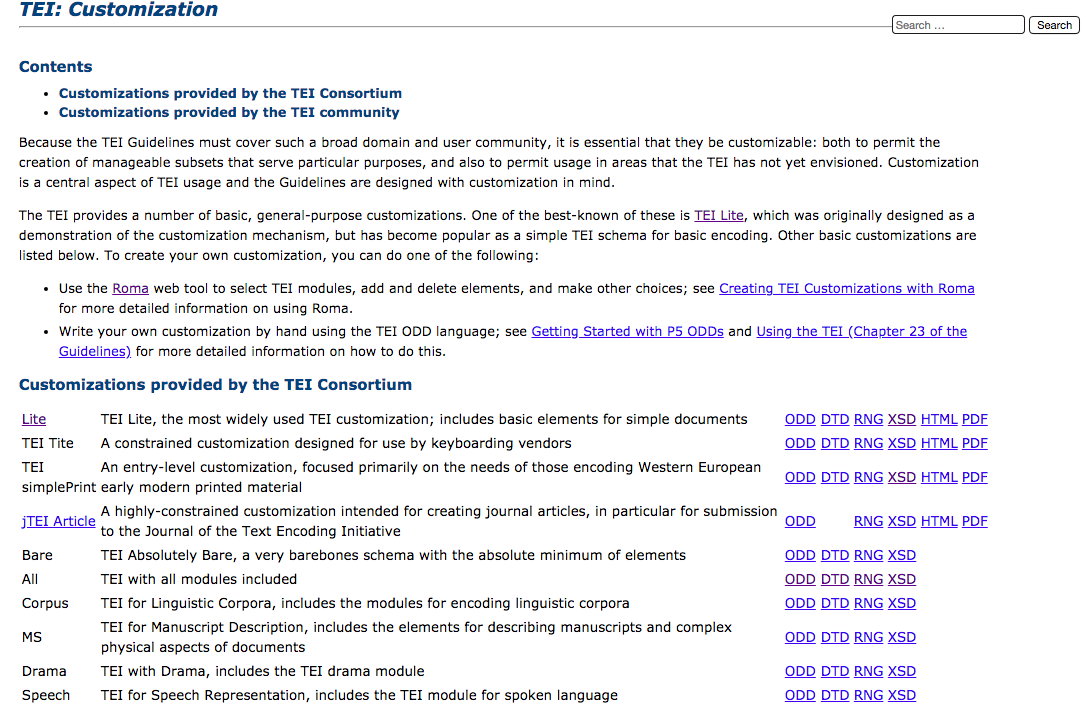
\includegraphics[width=.9\textwidth]{imgs/customization.png}
         \end{center}
       
        
    \end{frame}

    \begin{frame}
        \frametitle{Modularità e personalizzazione della TEI}
        \addtocounter{nframe}{1}

        \begin{block}{Creare da zero il proprio schema TEI}
                \begin{itemize}
                    \item TEI Roma: \url{http://www.tei-c.org/Roma/}
                    \item Selezione e restrizione del modello TEI
                    \item Estensione del modello TEI
                \end{itemize} 
        \end{block}
        
    \end{frame}

    \begin{frame}
        \frametitle{Modularità e personalizzazione della TEI}
        \addtocounter{nframe}{1}
        
        \textbf{Creazione di uno schema con l'applicazione Web Roma}

         \begin{center}
            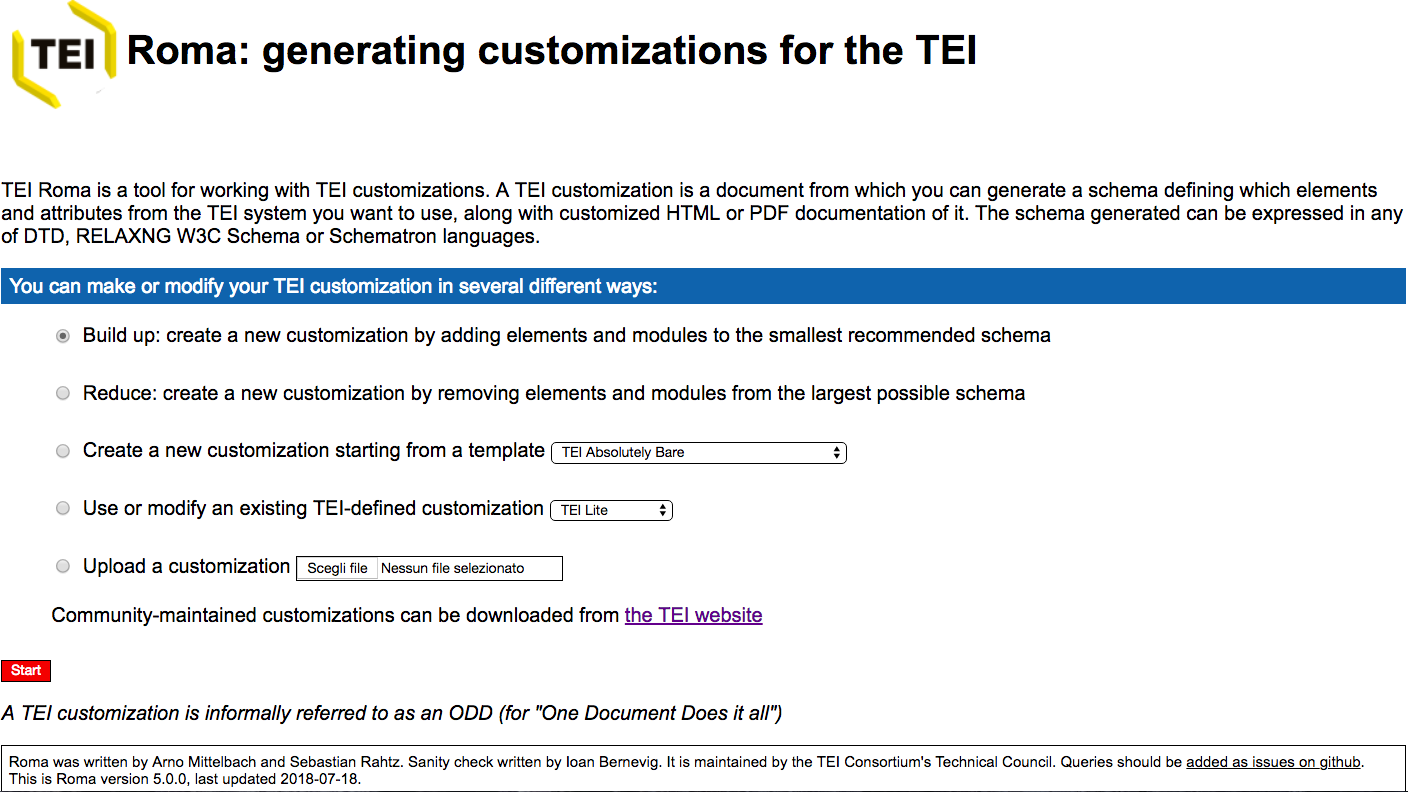
\includegraphics[width=.95\textwidth]{imgs/Roma1.png}
         \end{center}
       
        
    \end{frame}

    \begin{frame}
        \frametitle{Modularità e personalizzazione della TEI}
        \addtocounter{nframe}{1}
        
        \textbf{Passo 1: Inizializzare la personalizzazione}

         \begin{center}
            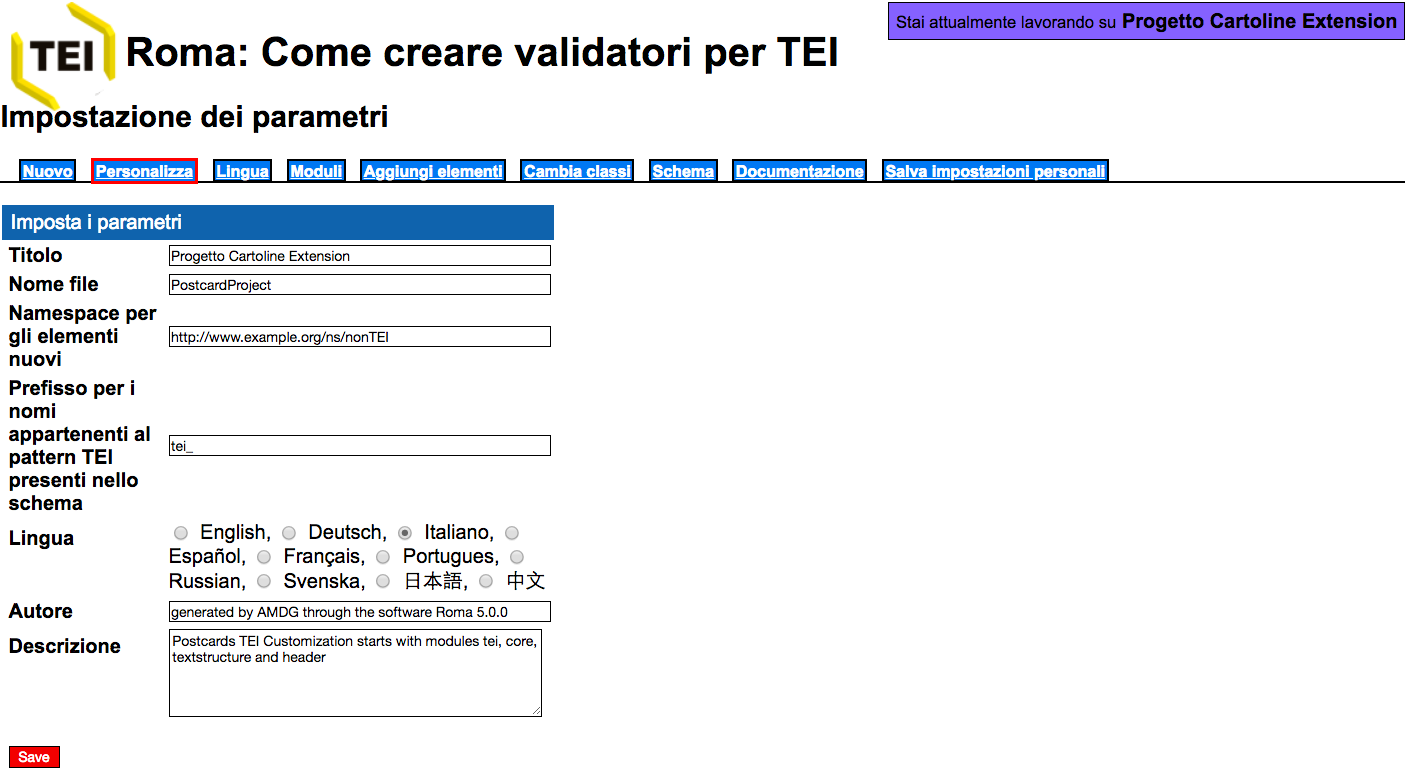
\includegraphics[width=.95\textwidth]{imgs/Roma2.png}
         \end{center}
       
        
    \end{frame}

%     ▪ New → scelta del punto di partenza
% ▪ Customize → personalizzazione metadati
% ▪ Language → lingua schema e documentazione
% ▪ Modules → scelta degli elementi TEI
% ▪ Add Elements → aggiunta elementi
% ▪ Change classes → gestione attributi
% ▪ Schema → generazione schema
% ▪ Documentation → creazione documentazione
% ▪ Save Customization → salvataggio file ODD


\begin{frame}
    \frametitle{Modularità e personalizzazione della TEI}
    \addtocounter{nframe}{1}
    
    \textbf{Passo 2: Selezionare la lingua dello schema}

     \begin{center}
        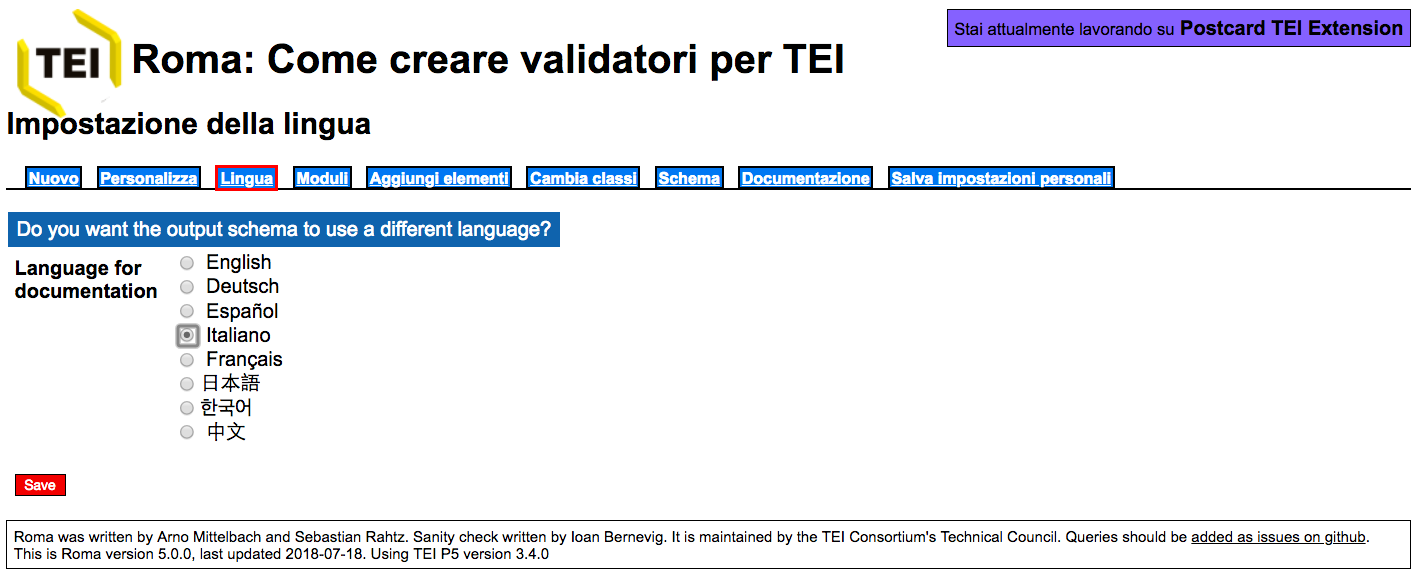
\includegraphics[width=.95\textwidth]{imgs/Roma3.png}
     \end{center}
   
    
\end{frame}

\begin{frame}
    \frametitle{Modularità e personalizzazione della TEI}
    \addtocounter{nframe}{1}
    
    \textbf{Passo 3: Selezionare i moduli da includere}

     \begin{center}
        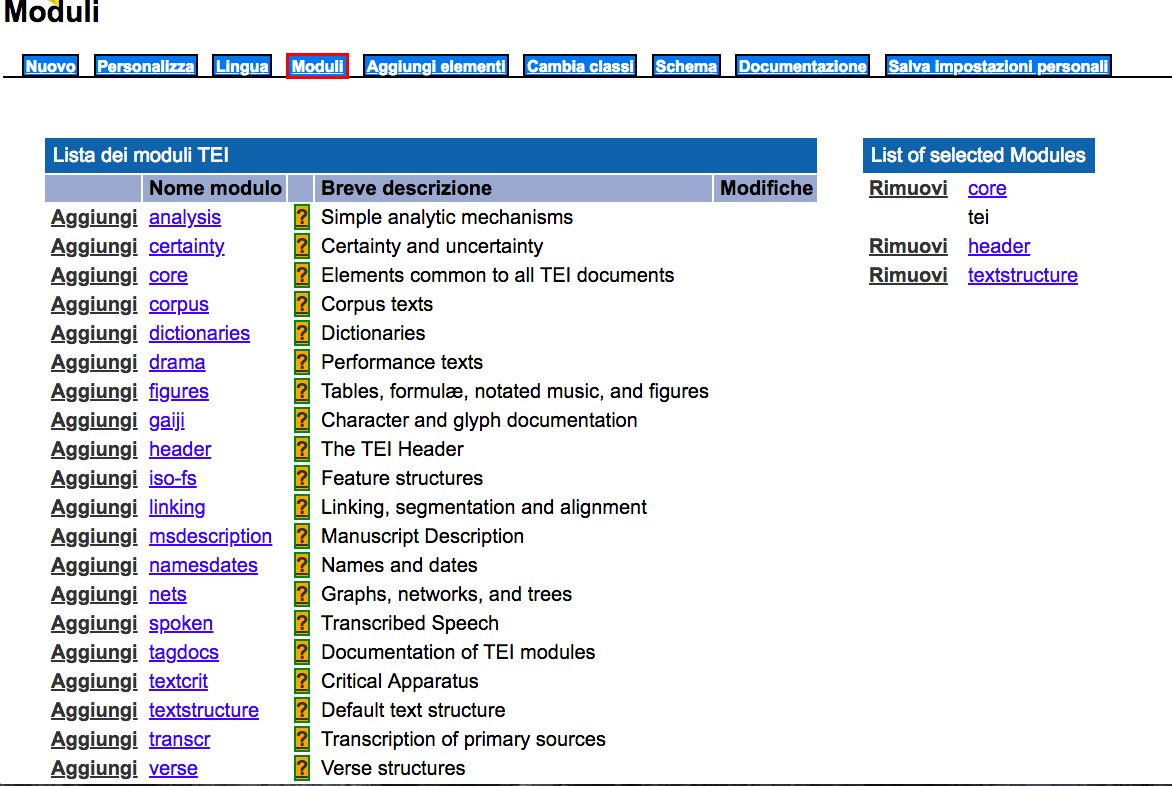
\includegraphics[width=.9\textwidth]{imgs/Roma4.png}
     \end{center}
   
    
\end{frame}

\begin{frame}
    \frametitle{Modularità e personalizzazione della TEI}
    \addtocounter{nframe}{1}
    
    \textbf{Passo 4:  Rimuovere i moduli già inclusi}


     \begin{center}
        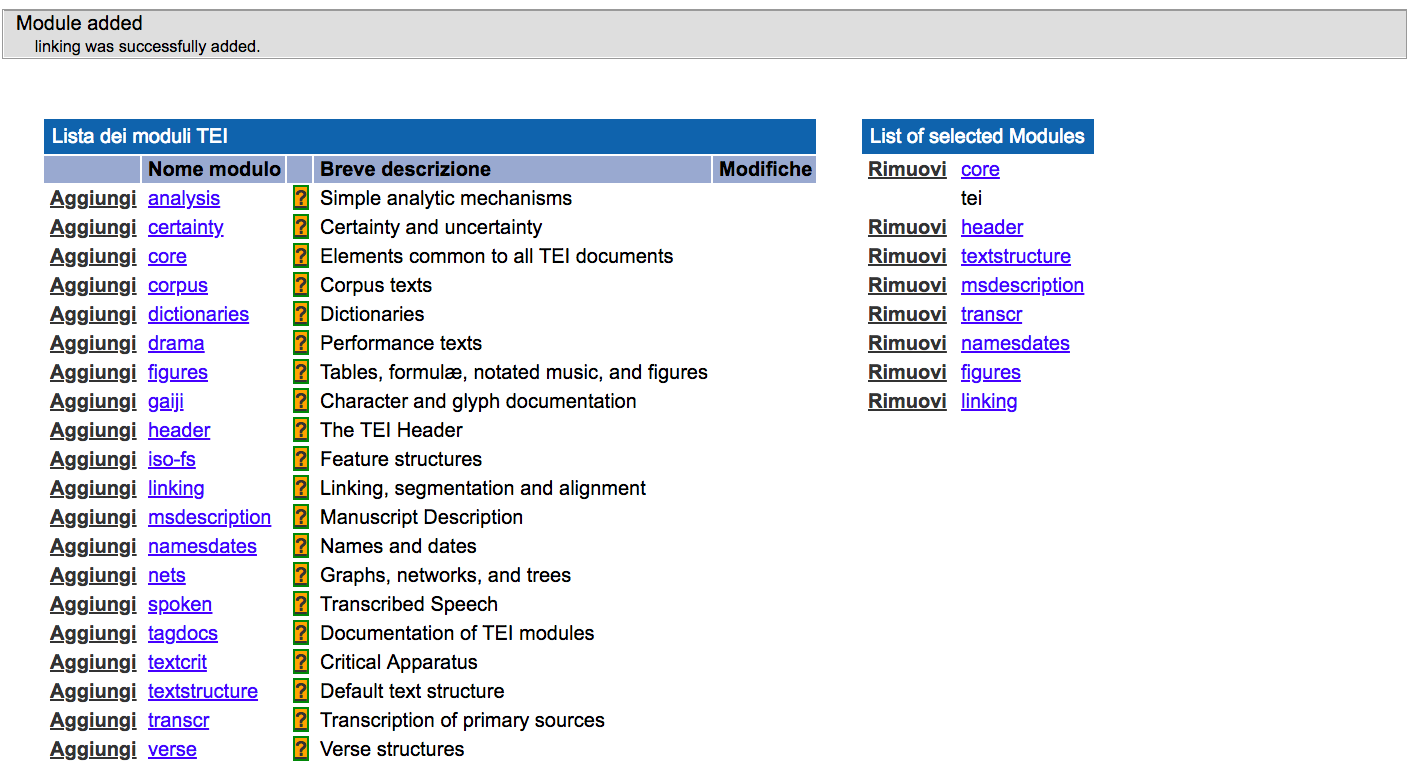
\includegraphics[width=.97\textwidth]{imgs/Roma5.png}
     \end{center}
   
    
\end{frame}

\begin{frame}
    \frametitle{Modularità e personalizzazione della TEI}
    \addtocounter{nframe}{1}
    
    
    \textbf{Passo 5: Selezionare gli elementi da includere/escludere}

     \begin{center}
        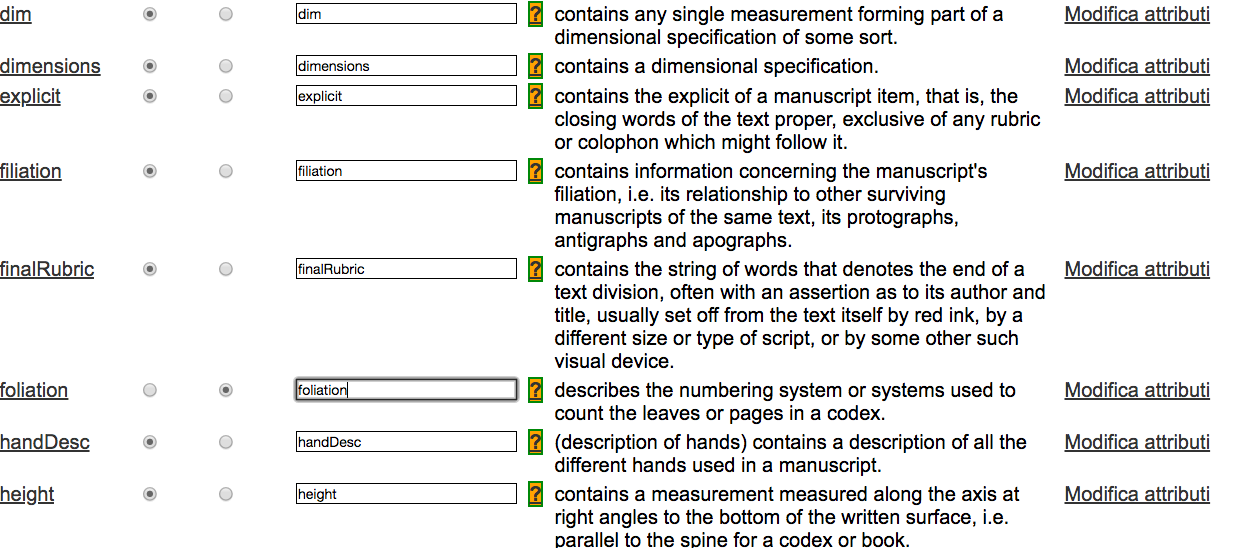
\includegraphics[width=.95\textwidth]{imgs/Roma6.png}
     \end{center}
   
    
\end{frame}

\begin{frame}
    \frametitle{Modularità e personalizzazione della TEI}
    \addtocounter{nframe}{1}
    
    \textbf{Passo 6: Selezionare gli attributi da includere/escudere}

     \begin{center}
        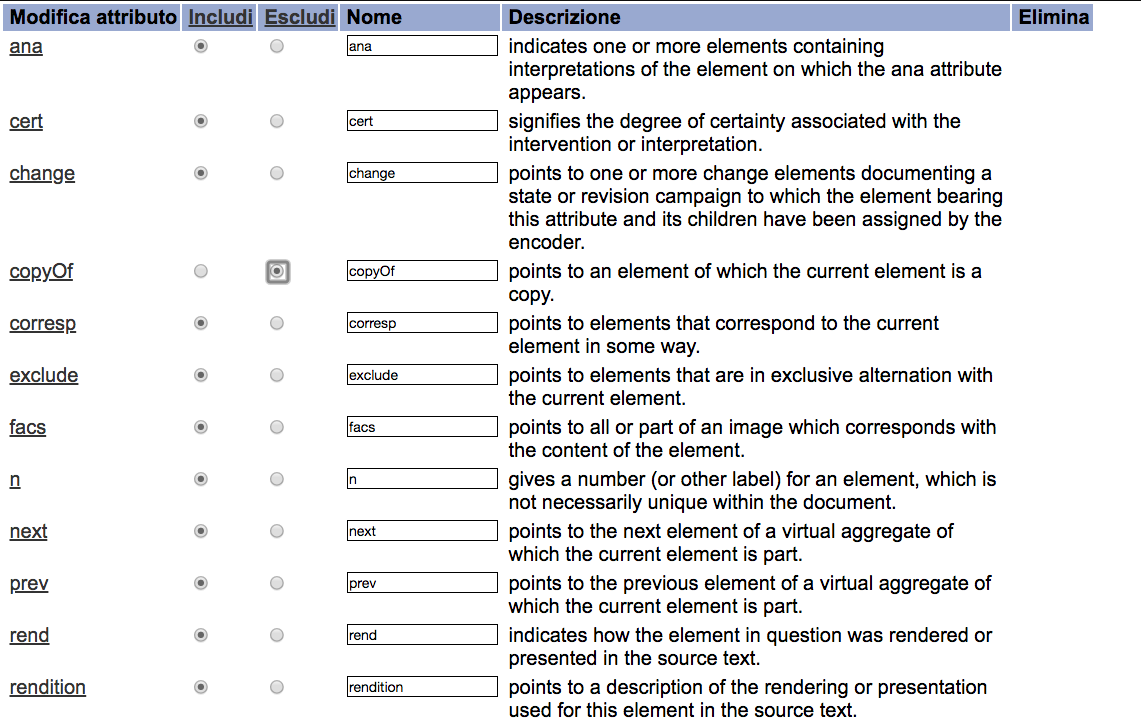
\includegraphics[width=.9\textwidth]{imgs/Roma7.png}
     \end{center}
   
    
\end{frame}

    
\begin{frame}
    \frametitle{Modularità e personalizzazione della TEI}
    \addtocounter{nframe}{1}
    
    \textbf{Passo 7: Aggiungere uno o più nuovi elementi}

     \begin{center}
        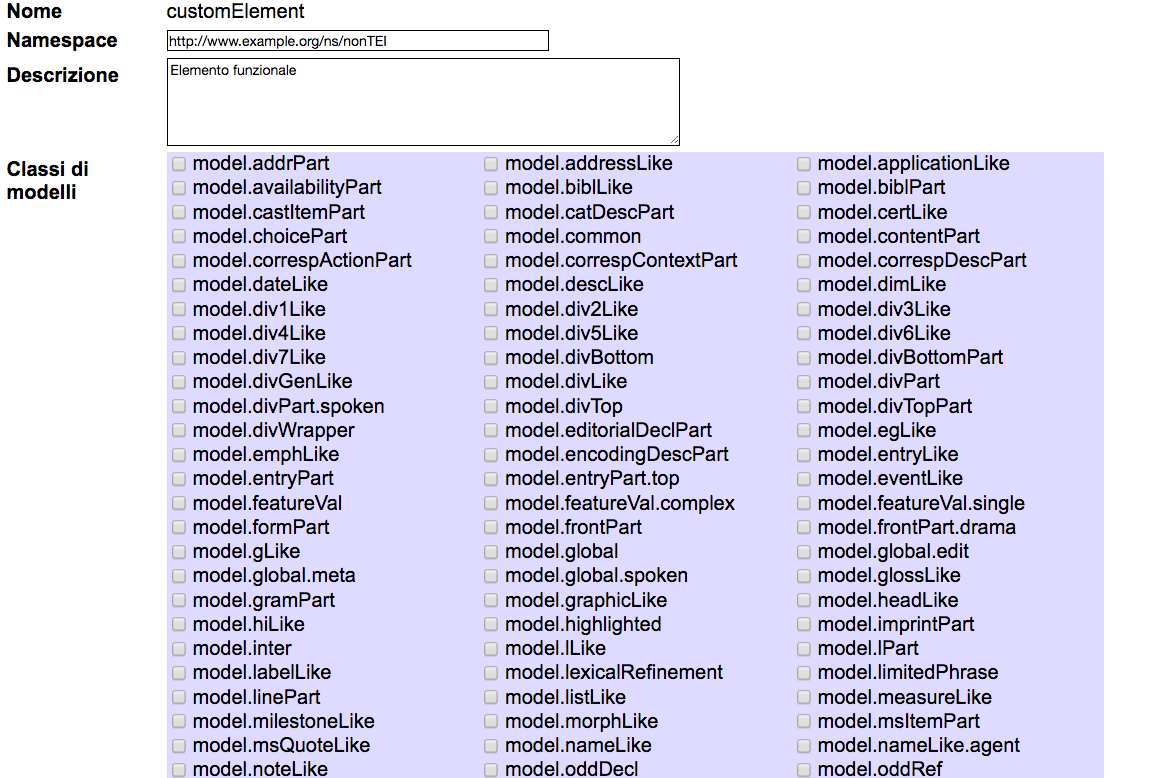
\includegraphics[width=.9\textwidth]{imgs/Roma9.png}
     \end{center}
    
\end{frame}
   
\begin{frame}
    \frametitle{Modularità e personalizzazione della TEI}
    \addtocounter{nframe}{1}
    
    \textbf{Passo 8: Aggiungere uno o più nuovi attributi}

     \begin{center}
        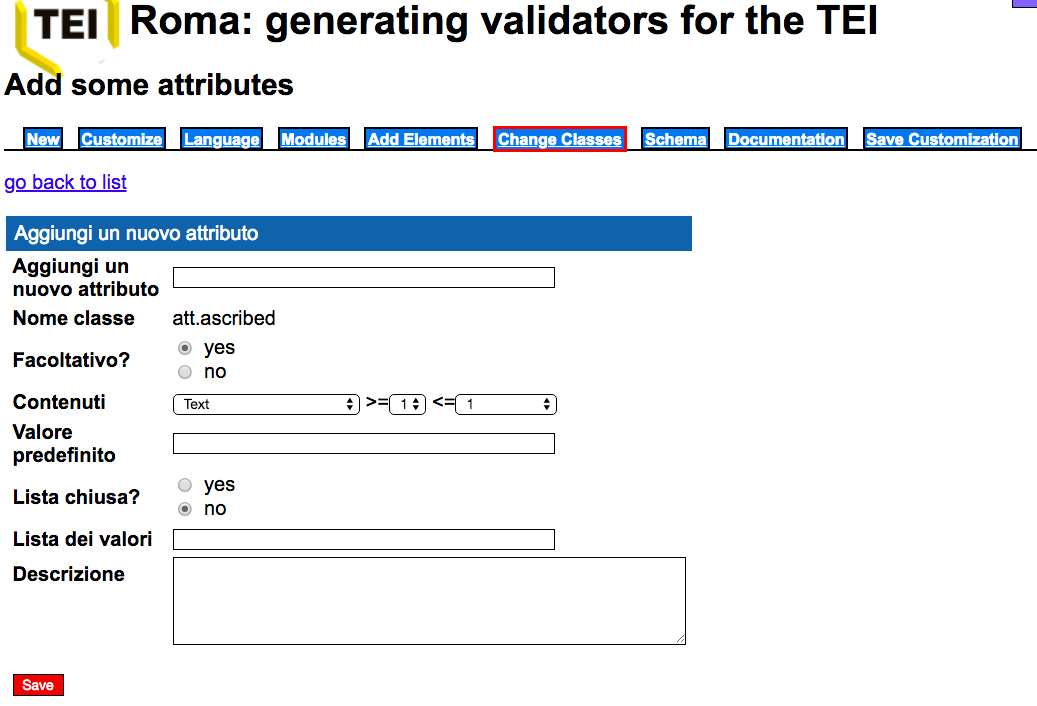
\includegraphics[width=.9\textwidth]{imgs/Roma14.png}
     \end{center}
     
    
\end{frame}
    
\begin{frame}
    \frametitle{Modularità e personalizzazione della TEI}
    \addtocounter{nframe}{1}

    \textbf{Passo 9: Validare gli elementi e gli attributi inclusi}

     \begin{center}
        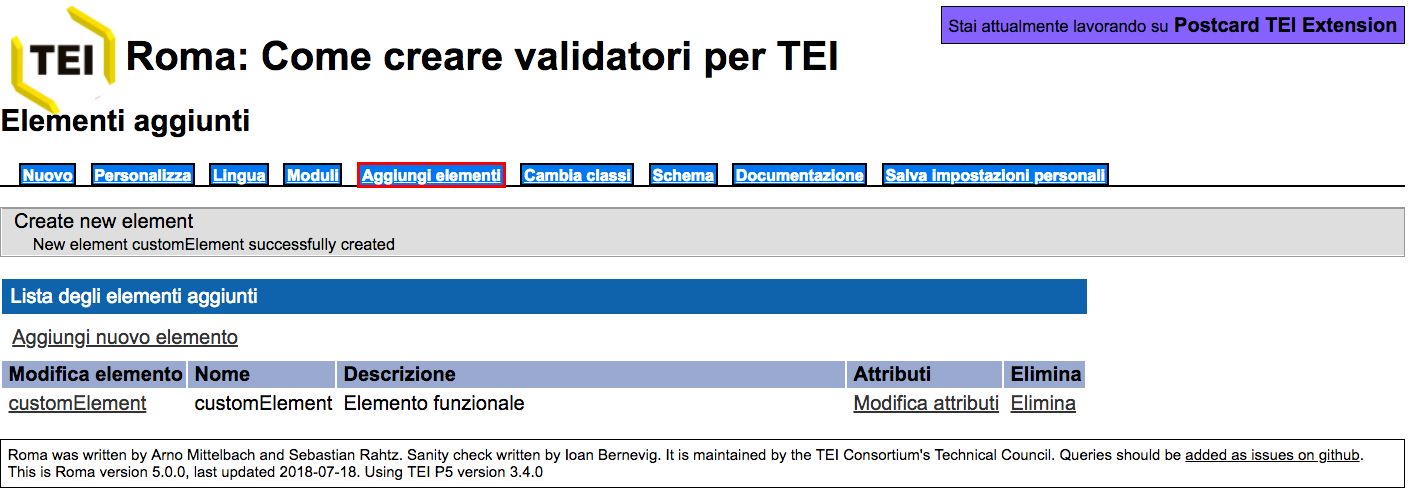
\includegraphics[width=.9\textwidth]{imgs/Roma8.png}
     \end{center}
   
    
\end{frame}


\begin{frame}
    \frametitle{Modularità e personalizzazione della TEI}
    \addtocounter{nframe}{1}
    
    \textbf{Passo 10: personalizzare le classi predefinite TEI }

     \begin{center}
        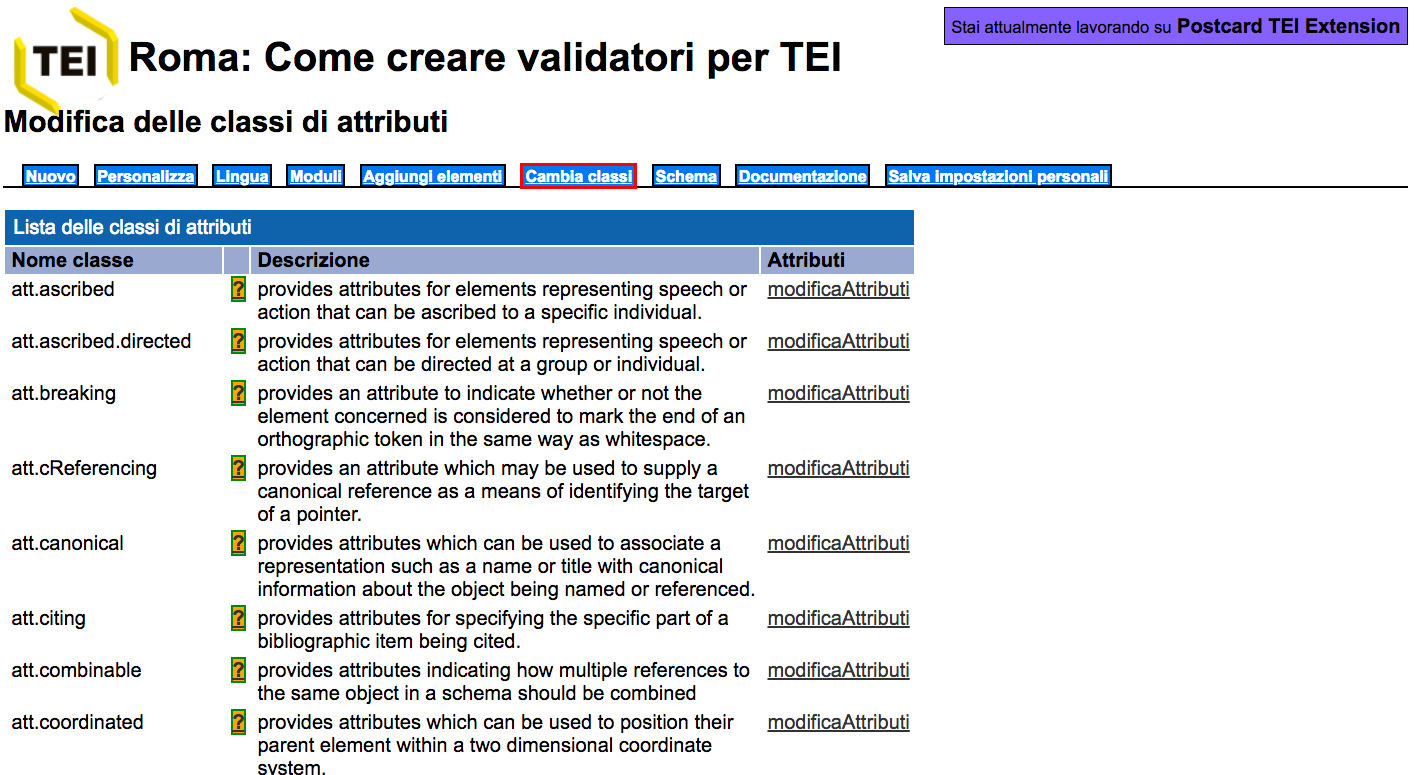
\includegraphics[width=.9\textwidth]{imgs/Roma10.png}
     \end{center}
   
    
\end{frame}

\begin{frame}
    \frametitle{Modularità e personalizzazione della TEI}
    \addtocounter{nframe}{1}
    
    \textbf{Passo 11: Modificare le classi predefinite TEI}

     \begin{center}
        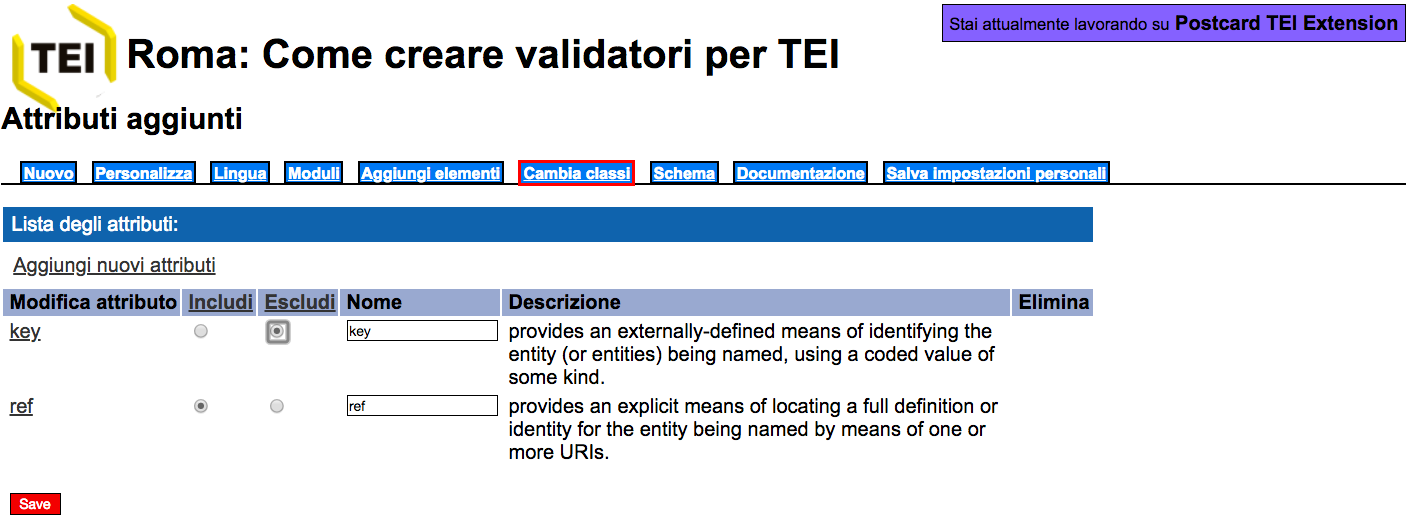
\includegraphics[width=.9\textwidth]{imgs/Roma11.png}
     \end{center}
   
    
\end{frame}

\begin{frame}
    \frametitle{Modularità e personalizzazione della TEI}
    \addtocounter{nframe}{1}
   
   
    \textbf{Passo 12: Generazione dello schema}

     \begin{center}
        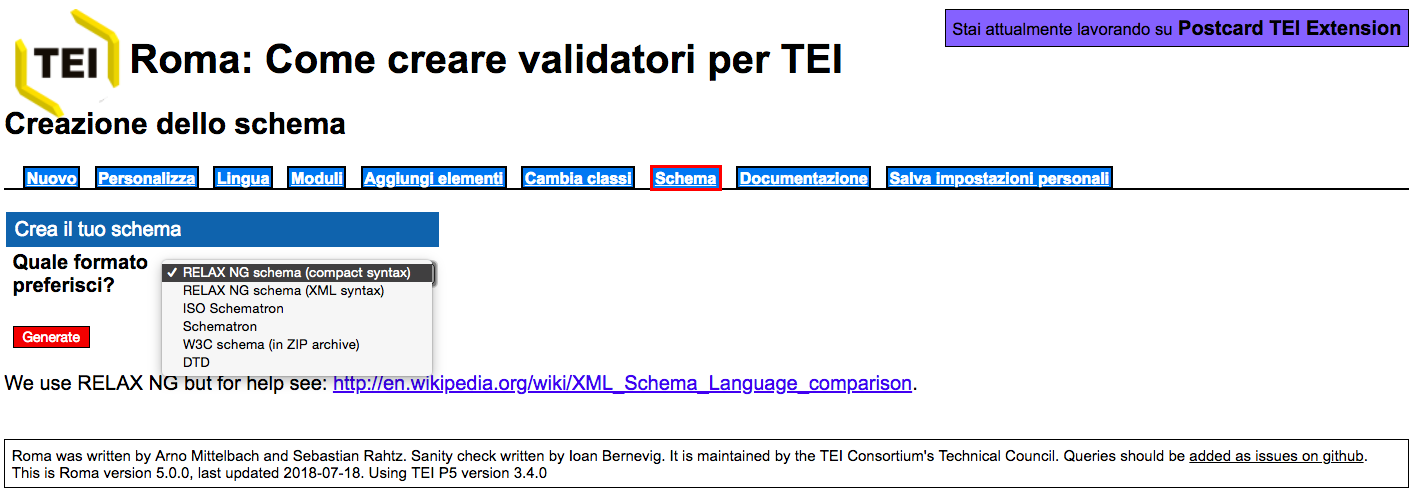
\includegraphics[width=.9\textwidth]{imgs/Roma12.png}
     \end{center}
   
    
\end{frame}

\begin{frame}
    \frametitle{Modularità e personalizzazione della TEI}
    \addtocounter{nframe}{1}
    
    \textbf{Passo 13: Generazione della documentazione}

     \begin{center}
        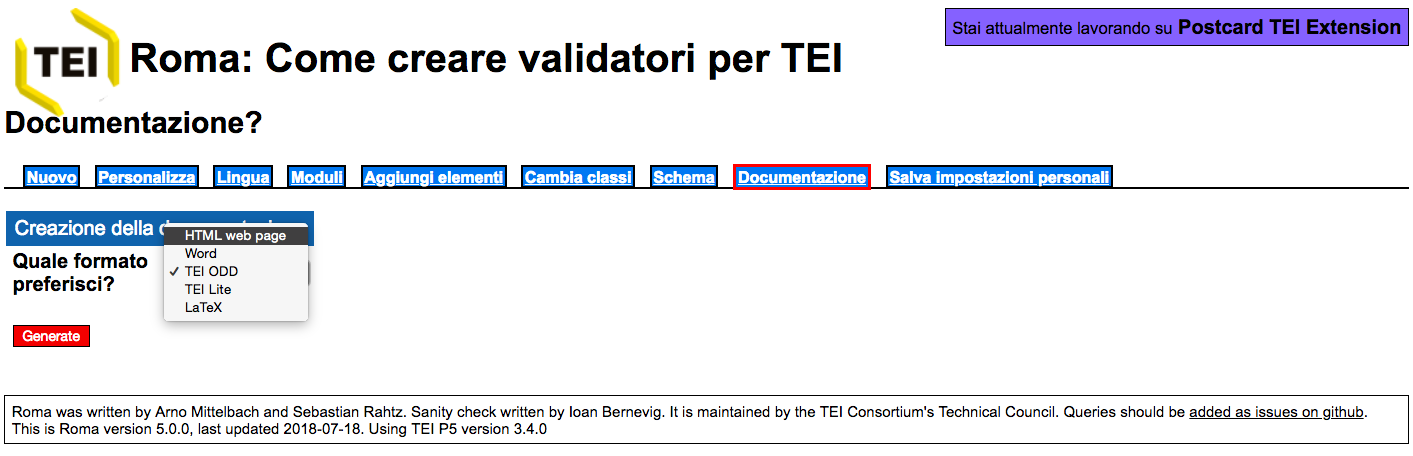
\includegraphics[width=.95\textwidth]{imgs/Roma13.png}
     \end{center}
    
\end{frame}

\begin{frame}
    \frametitle{Modularità e personalizzazione della TEI}
    \addtocounter{nframe}{1}
    
    \textbf{Passo 14: Generazione del documento ODD}

     \begin{center}
        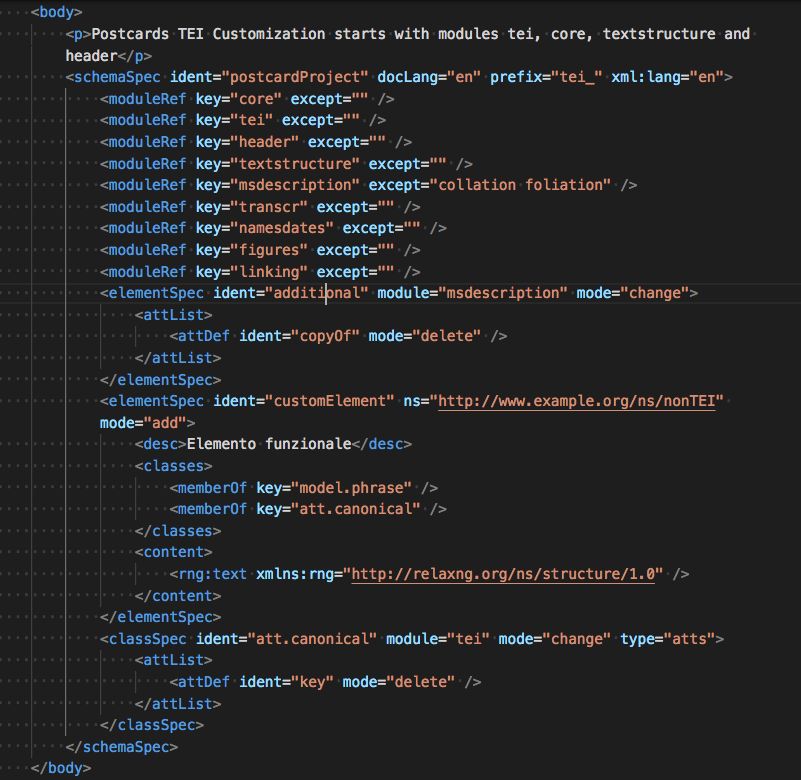
\includegraphics[width=.65\textwidth]{imgs/CustomizationODD.png}
     \end{center}
    
\end{frame}


\begin{frame}
    \frametitle{Modularità e personalizzazione della TEI}
    \addtocounter{nframe}{1}
    
    \textbf{Documento ODD}

     \begin{center}
        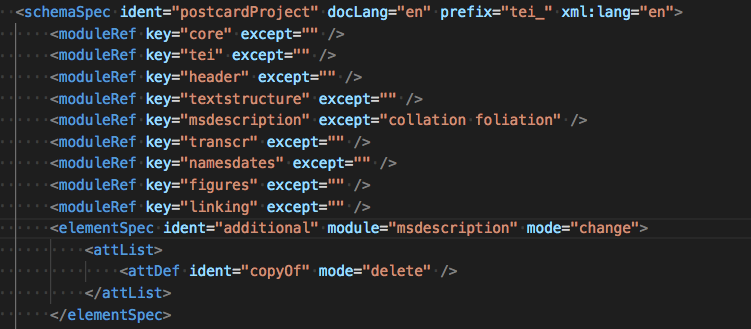
\includegraphics[width=.97\textwidth]{imgs/CustomizationODD-1.png}
     \end{center}
    
\end{frame}

\begin{frame}
    \frametitle{Modularità e personalizzazione della TEI}
    \addtocounter{nframe}{1}
    
    \textbf{Documento ODD}

     \begin{center}
        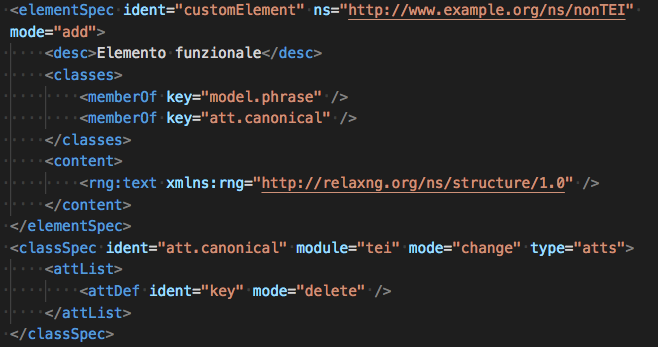
\includegraphics[width=.97\textwidth]{imgs/CustomizationODD-2.png}
     \end{center}
    
\end{frame}

\begin{frame}
    \frametitle{Modularità e personalizzazione della TEI}
    \addtocounter{nframe}{1}
    
    \textbf{Schema dtd con le personalizzazioni}

     \begin{center}
        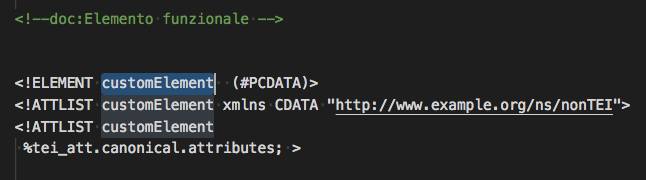
\includegraphics[width=.97\textwidth]{imgs/TEI-Custom-DTD.png}
     \end{center}
   
    
\end{frame}

\begin{frame}
    \frametitle{Modularità e personalizzazione della TEI}
    \addtocounter{nframe}{1}
    
    \textbf{Schema dtd con le personalizzazioni}

     \begin{center}
        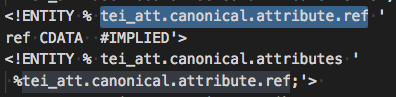
\includegraphics[width=.9\textwidth]{imgs/TEI-Custom-DTD-2.png}
     \end{center}
   
    
\end{frame}



\begin{frame}
    \frametitle{Modularità e personalizzazione della TEI}
    \addtocounter{nframe}{1}

    \begin{block}{Approfondimenti}
            \begin{itemize}
                \item Customizing the TEI with Roma
                \item [] \url{http://www.tei-c.org/Guidelines/Customization/use_roma.xml}
                \item Getting Started with P5 ODDs
                \item [] \url{http://www.tei-c.org/Guidelines/Customization/odds.xml}
                \item TEI By Example: Customising TEI, ODD, Roma
                \item [] \url{http://teibyexample.org/modules/TBED08v00.htm}
            \end{itemize} 
    \end{block}

\end{frame}
